\documentclass[11pt,
  letterpaper,
  openany,
  toc=bibliography,
  idxtotoc,
  bookmarks]{labbook}

\usepackage[utf8]{inputenc}
\usepackage[T1]{fontenc}
\usepackage[spanish]{babel}

\usepackage[margin=2.5cm]{geometry}
\usepackage{microtype}
\usepackage{graphicx}
\usepackage{amsmath,amssymb}
\usepackage{csquotes}
\usepackage{booktabs}
\usepackage{enumitem}
\usepackage{authblk}
\usepackage[spanish]{cleveref}
\usepackage[dvipsnames]{xcolor}
\usepackage{pgfplotstable}
\usepackage{siunitx}
\usepackage{subcaption}
\usepackage{multirow}
\usepackage{float}

\pgfplotsset{compat=1.18}
\pgfkeys{/pgf/number format/1000 sep={\,}}

\AtBeginDocument{\decimalpoint}
\renewcommand{\arraystretch}{1.2}
\sisetup{group-digits=true,
  group-separator={\,},
  separate-uncertainty}

\usepackage[backend=biber,style=numeric]{biblatex}
\addbibresource{./references-pre-project.bib}

\usepackage{pdfbase}
\pdfinfo{
  /Title (Electron Beam)
  /Author (Sebastián Rodríguez, Laura Torres, Julián Ávila)
  /Creator (LaTeX with labbook class)
}

\title{\textbf{Rayo de Electrones} \\
Bitácora de Laboratorio}
\author{Sebastian Rodríguez \and Laura Torres \and Julian Avila}
\affil{Universidad Distrital Francisco José de Caldas}
\date{}

\begin{document}

\maketitle

\tableofcontents

\labday{Miércoles 4, Junio 2025}

\section{Montaje Experimental: Deflexión de un Haz de Electrones con Bobinas de Helmholtz}
Este montaje experimental tiene como objetivo \textbf{demostrar la deflexión de un haz de electrones} bajo la influencia de campos magnéticos generados por pares de bobinas de Helmholtz. Aunque el concepto de partida fue simular un experimento de Stern-Gerlach, el diseño actual se centra en la observación de la trayectoria del haz de electrones al pasar por campos magnéticos controlados.

---

\subsection{Componentes del Montaje}
El sistema se compone principalmente de los siguientes elementos:
\begin{itemize}
    \item \textbf{Cañón de Electrones (Leibold):} Genera un haz de electrones colimado. Se opera a un potencial de aceleración de aproximadamente \textbf{3.1 kV a 4.3 kV}. El haz de electrones emerge del cañón ya enfocado y con una dirección definida.
    \item \textbf{Tubo de Rayos Catódicos (Leibold):} Es el recipiente de vacío por donde viaja el haz de electrones desde el cañón hasta la pantalla.
    \item \textbf{Pares de Bobinas de Helmholtz (Leibold):} Se utilizan dos pares de bobinas coaxiales, cada par alimentado por una \textbf{fuente de corriente variable de hasta 3 Amperios}. Estas bobinas son fundamentales para generar los campos magnéticos que interactúan con el haz de electrones.
    \begin{itemize}
        \item \textbf{Dimensiones Aproximadas de las Bobinas:}
        \begin{itemize}
            \item Radio ($R$): Aproximadamente \textbf{6.5 cm}.
            \item Número de Giros por Bobina ($N$): Aproximadamente \textbf{320 giros}.
        \end{itemize}
    \end{itemize}
    \item \textbf{Fuentes de Corriente Variables:} Son esenciales para suministrar y controlar la corriente (hasta 3A) que circula por cada par de bobinas. Permiten ajustar la magnitud del campo magnético generado.
    \item \textbf{Pantalla Fluorescente:} Ubicada al final de la trayectoria del haz de electrones dentro del tubo, donde el impacto de los electrones genera un punto luminoso, permitiendo la observación visual de la trayectoria y deflexión del haz.
\end{itemize}

---

\subsection{Disposición del Montaje}
El cañón de electrones se alinea de manera que el haz de electrones colimado pase directamente a través del centro de las bobinas de Helmholtz. Los dos pares de bobinas se colocan coaxialmente, es decir, sus ejes se encuentran sobre la misma línea, la cual coincide con la trayectoria inicial del haz de electrones. El haz emerge del cañón, atraviesa el espacio entre los pares de bobinas y, finalmente, incide sobre la pantalla fluorescente. como se muestra en la siguiente imagen.

\begin{figure}[htbp]
    \centering
    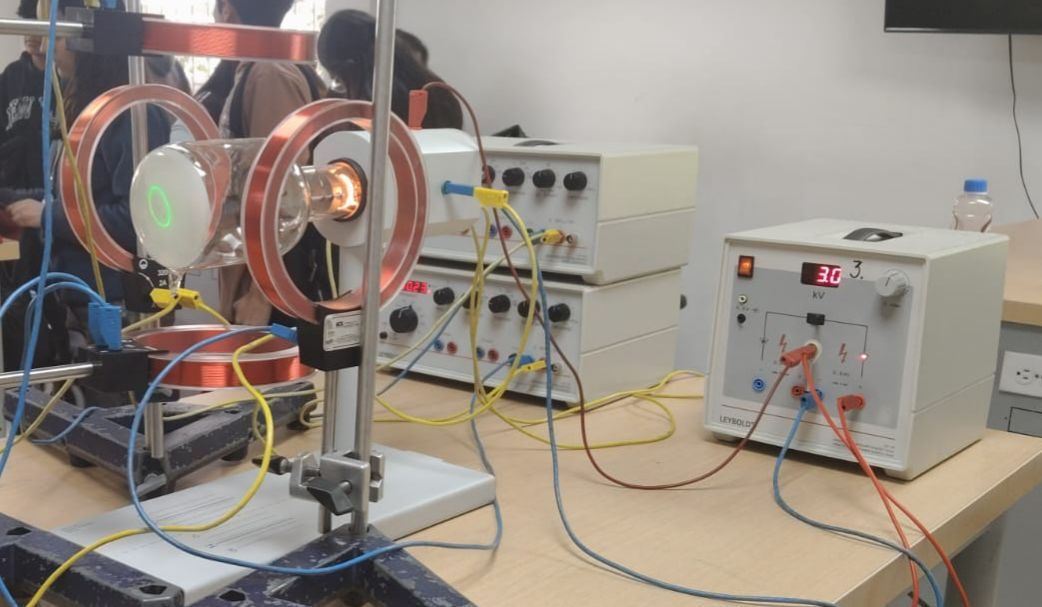
\includegraphics[width=0.8\textwidth]{Sections/Figures/Montaje.jpeg}
    \caption{Montaje experimental.}
    \label{fig:nombre_descriptivo_de_la_imagen}
\end{figure}

---

\subsection{Configuraciones de las Bobinas y Generación de Campo Magnético}
La versatilidad de este montaje radica en la capacidad de configurar las bobinas de dos maneras distintas para generar diferentes campos magnéticos:

\subsubsection{1. Configuración Helmholtz (Campo Aditivo)}
\begin{itemize}
    \item \textbf{Descripción:} En esta configuración, la corriente fluye en la \textbf{misma dirección} a través de ambas bobinas de cada par (y también entre los dos pares coaxiales si están siendo usados en conjunto de esta forma).
    \item \textbf{Campo Magnético Generado:} Esta disposición produce un \textbf{campo magnético uniforme y aditivo} en la región central entre las bobinas. Este campo es aproximadamente paralelo al eje de las bobinas.
    \item \textbf{Efecto en el Haz de Electrones:} Un campo uniforme y perpendicular a la velocidad de los electrones causará una \textbf{deflexión circular} del haz.
\end{itemize}

\subsubsection{2. Configuración Anti-Helmholtz (Campo Sustractivo/Gradiente)}
\begin{itemize}
    \item \textbf{Descripción:} Para esta configuración, la corriente se invierte en una de las bobinas de cada par (o entre los pares si se usan para generar un gradiente axial), de modo que fluye en \textbf{direcciones opuestas} entre ellas.
    \item \textbf{Campo Magnético Generado:} Esta disposición crea un \textbf{campo magnético con un fuerte gradiente} en la región central. El campo es nulo en el punto medio exacto entre las bobinas y aumenta en magnitud a medida que uno se aleja de este punto central, con direcciones opuestas a cada lado.
    \item \textbf{Efecto en el Haz de Electrones:} Un gradiente de campo magnético perpendicular a la trayectoria del haz puede generar \textbf{fuerzas variables} sobre los electrones, resultando en patrones de deflexión más complejos, potencialmente extendiendo el punto luminoso en la pantalla.
\end{itemize}

---

\subsection{Funcionamiento y Observaciones}
Las fuentes de corriente variables permiten ajustar la magnitud del campo magnético generado por las bobinas. Durante el experimento, se aplicaron \textbf{señales de corriente tipo seno, rampa y cuadrada} con \textbf{frecuencias nunca superiores a los 100 Hz}. La interacción del haz de electrones con el campo magnético resultante produce patrones luminosos en la pantalla fluorescente. Se observaron figuras dinámicas en la pantalla que recordaban a \textbf{figuras de Lissajous}, pero que variaban en el tiempo debido a la modulación de los campos magnéticos. Un análisis posterior detallará las características de estas figuras y su relación con las configuraciones y frecuencias de las bobinas.

Este montaje permite una clara demostración de cómo los campos magnéticos, generados en diferentes configuraciones, pueden influir en la trayectoria de partículas cargadas como los electrones.


\labday{Jueves 5, Junio 2025}

\section{Análisis posterior del montaje y sugerencia de simulación}

Como el montaje tenía las dos posibles configuraciones donde las bobinas pueden estar aditivas (\textbf{Helmholtz}) o sustractivas (\textbf{Anti-Helmholtz}), la idea era ver la morfología del campo magnético en cada caso para entender el comportamiento del haz de electrones. Por ende, se graficaron, para unas bobinas arbitrarias, los campos en el plano $x,y$ al que pertenecen los vectores normales de las bobinas, es decir, el plano perpendicular al haz.

\begin{figure}[H]
    \centering
    \begin{minipage}[b]{0.48\textwidth}
        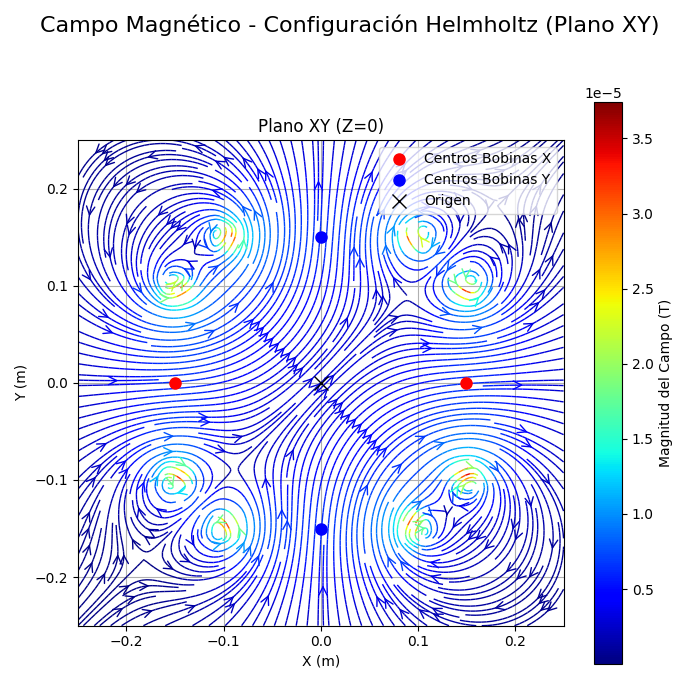
\includegraphics[width=\linewidth]{Sections/Figures/helmholtz_xy_field.png}
        \caption{Bobinas en  Helmholtz.}
        \label{fig:helmholtz_xy_field}
    \end{minipage}
    \hfill
    \begin{minipage}[b]{0.48\textwidth}
        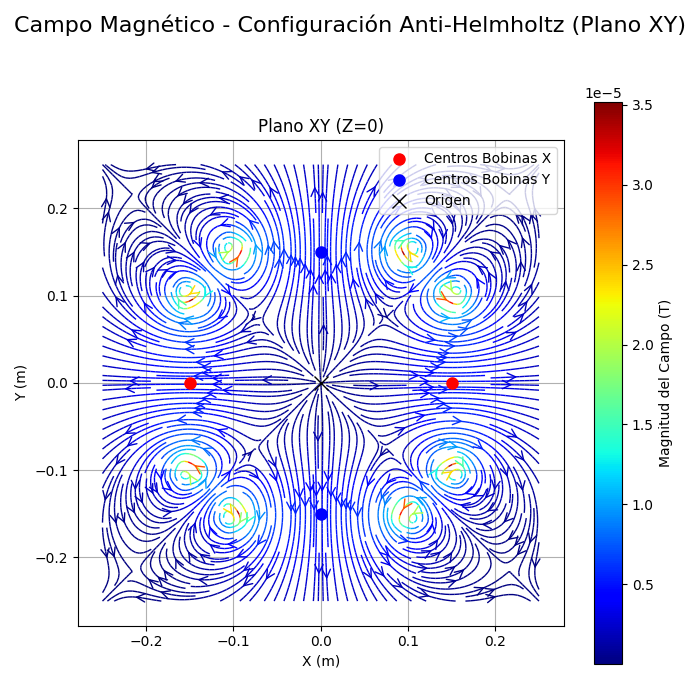
\includegraphics[width=\linewidth]{Sections/Figures/antihelmholtz_xy_field.png}
        \caption{Bobinas en  Anti-Helmholtz.}
        \label{fig:antihelmholtz_xy_field}
    \end{minipage}
    %\caption{Morfología del campo magnético en el plano $x,y$ para las configuraciones Helmholtz y Anti-Helmholtz.}
    \label{fig:campos_bobinas}
\end{figure}

Posteriormente, y dado que se tenía información sobre el comportamiento del campo en cortes del volumen generado por las bobinas, se procedió a graficar el esquema de la simulación basándose en estos campos, como se puede ver en la siguiente gráfica que representa la trayectoria del haz a través de los campos generados.

\begin{figure}[H]
    \centering
    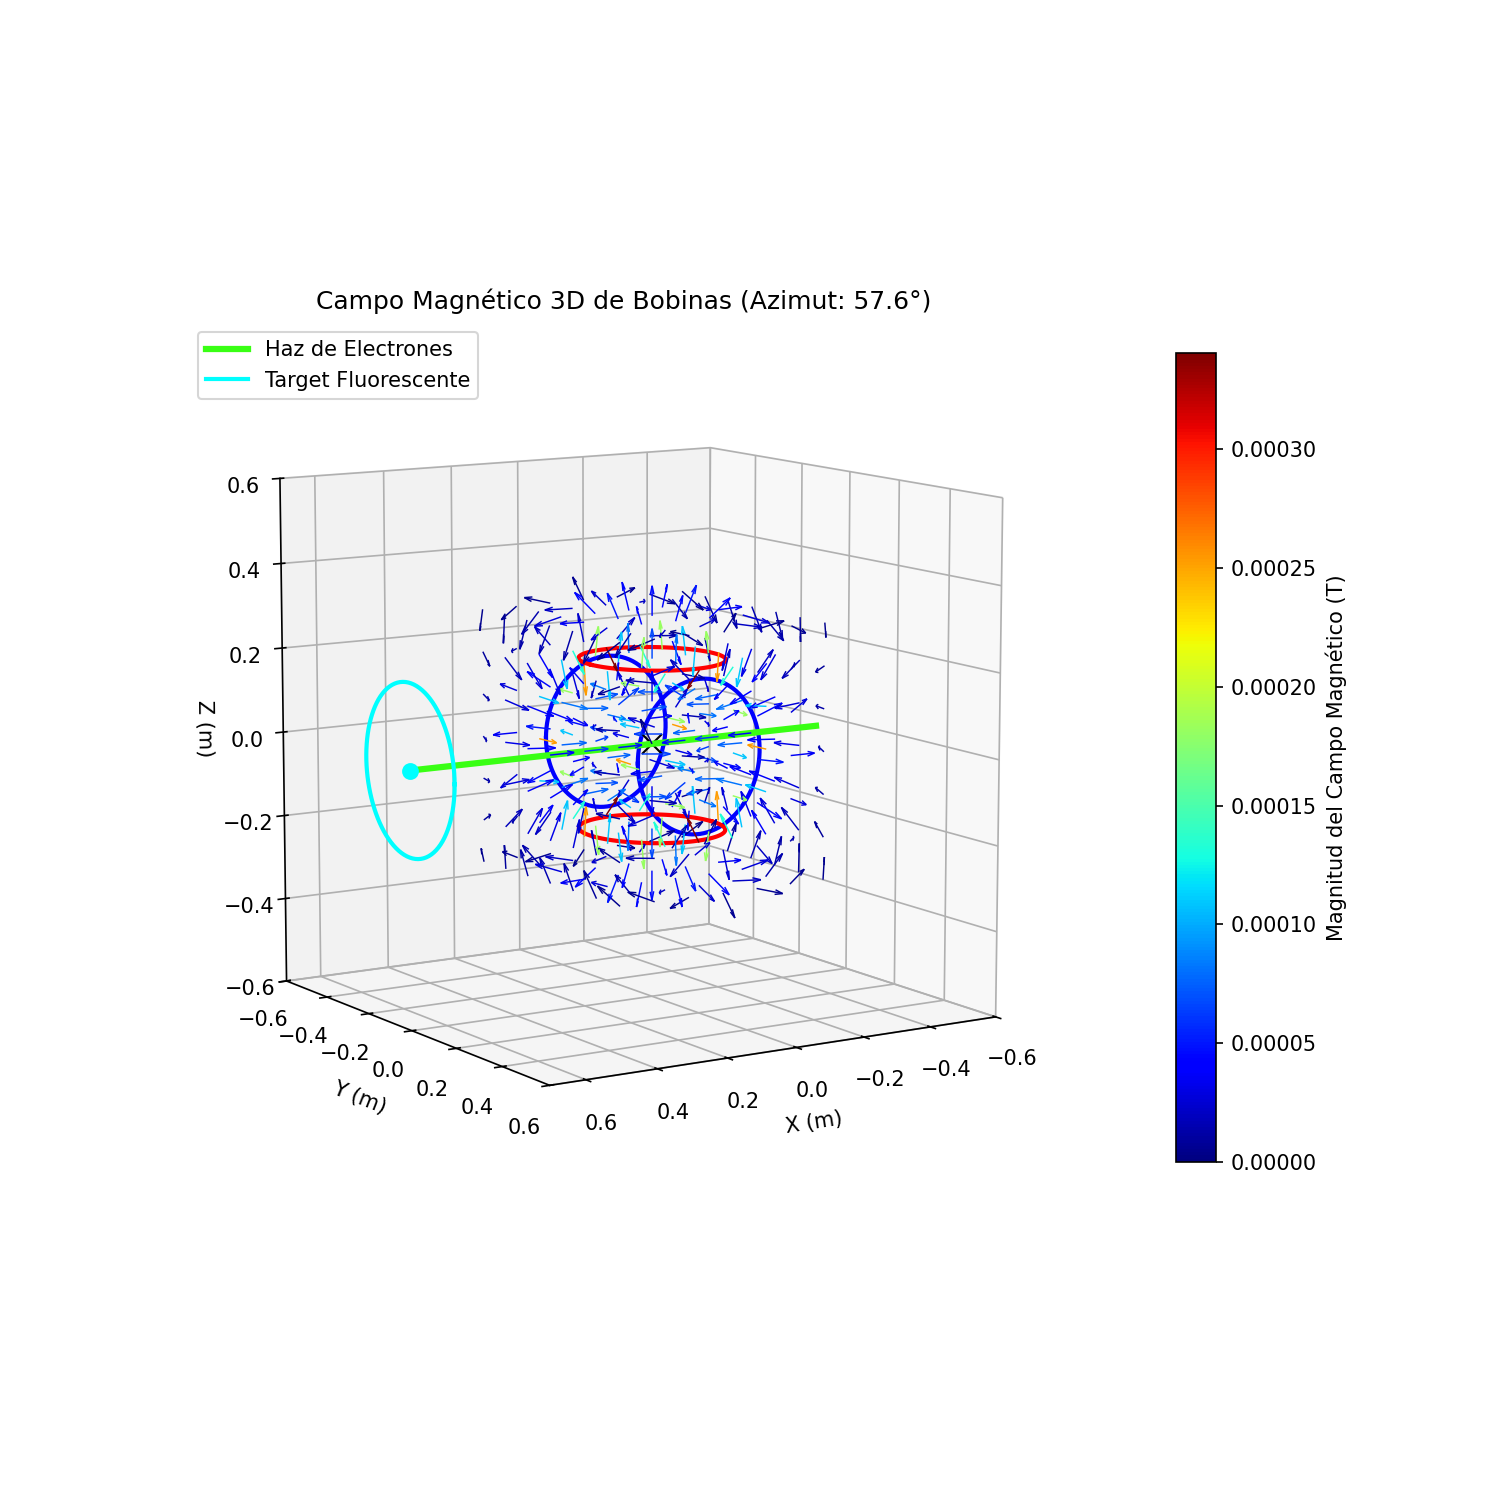
\includegraphics[width=0.8\textwidth]{Sections/Figures/frame_azim_057.6.png}
    \caption{Trayectoria del haz para la simulación.}
    \label{fig:trayectoria_haz_simulacion}
\end{figure}

Finalmente, se realizaron las primeras especulaciones sobre si los \textbf{campos eléctricos inducidos} en el montaje tendrían influencia en la modificación del comportamiento del haz, y si estos deberían considerarse como un factor importante en la simulación. También, tras una investigación sobre el montaje, se pudo observar su similitud con un \textbf{Stern-Gerlach}, donde una característica de su campo magnético es que suelen ser campos no uniformes, generados en muchas ocasiones con sistemas de cuadrupolos. Por lo tanto, se propone que, para optimizar las simulaciones, se contemple la posibilidad de generar los campos con \textbf{dipolos} o \textbf{cuadrupolos}.

\labday{Lunes 8, Junio 2025}

\section{Viabilidad de dipolos y cuadrupolos para la simulación del haz}

Para poder ver el \textbf{comportamiento de los campos} de las dos configuraciones contempladas, generados por dipolos y cuadrupolos, se crearon las siguientes gráficas:

\begin{figure}[H] % Uso de [H] para mantener la figura en su posición
    \centering
    % Ajusta el ancho de minipage para que quepan dos imágenes (ej. 0.48\textwidth)
    % y usa 'trim' y 'clip' para cortar la imagen si es necesario
    \begin{minipage}[b]{0.48\textwidth} % Ancho ajustado para que quepan dos imágenes
        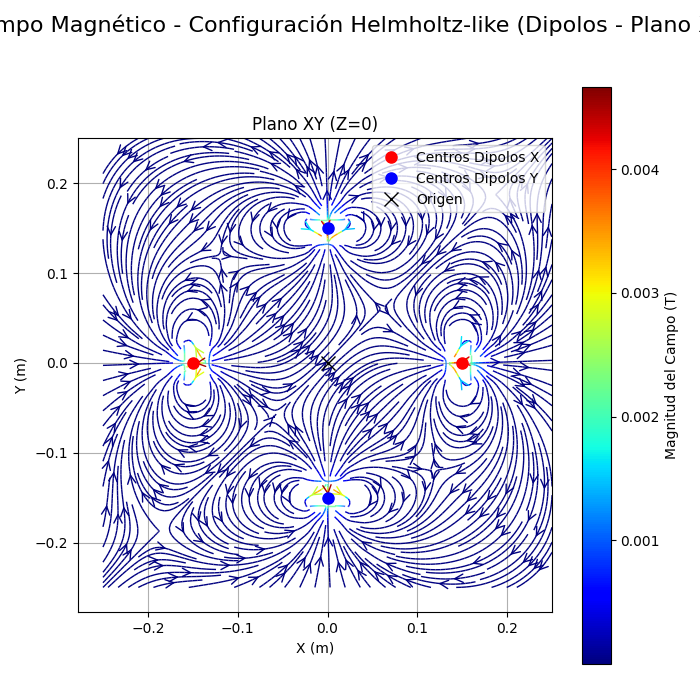
\includegraphics[width=\linewidth, trim={0cm 2cm 0cm 1cm}, clip]{Sections/Figures/helmholtz_dipoles_xy_field.png} % Valores de trim/clip de ejemplo
        \caption{Dipolos en Helmholtz.}
        \label{fig:helmholtz_dipoles_xy_field}
    \end{minipage}
    \hfill
    \begin{minipage}[b]{0.48\textwidth} % Ancho ajustado para que quepan dos imágenes
        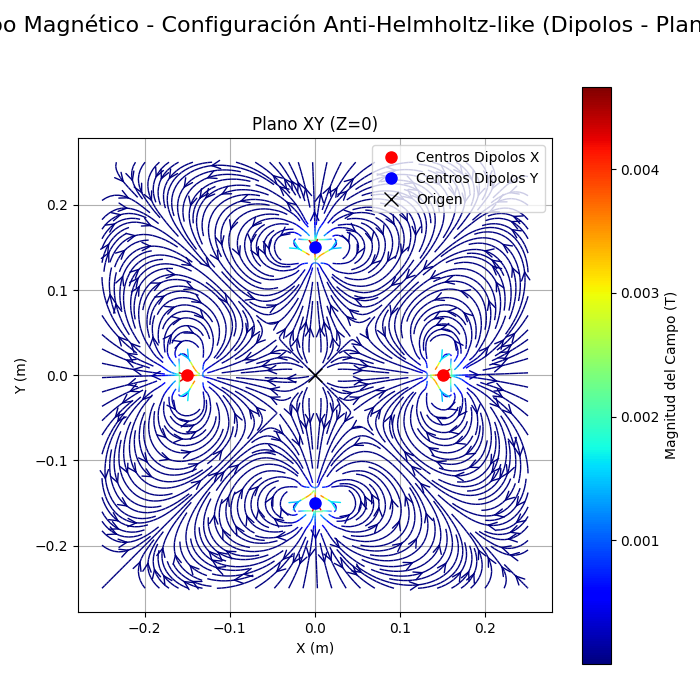
\includegraphics[width=\linewidth, trim={0cm 2cm 0cm 1cm}, clip]{Sections/Figures/antihelmholtz_dipoles_xy_field.png} % Valores de trim/clip de ejemplo
        \caption{Dipolos en Anti-Helmholtz.}
        \label{fig:antihelmholtz_dipoles_xy_field}
    \end{minipage}
    \caption{Morfología del campo magnético en el plano $x,y$ generado por dipolos en configuraciones Helmholtz y Anti-Helmholtz.}
    \label{fig:campos_dipolos}
\end{figure}

\begin{figure}[H] % Uso de [H] para mantener la figura en su posición
    \centering
    % Ajusta el ancho de minipage y usa 'trim' y 'clip'
    \begin{minipage}[b]{0.48\textwidth} % Ancho ajustado
        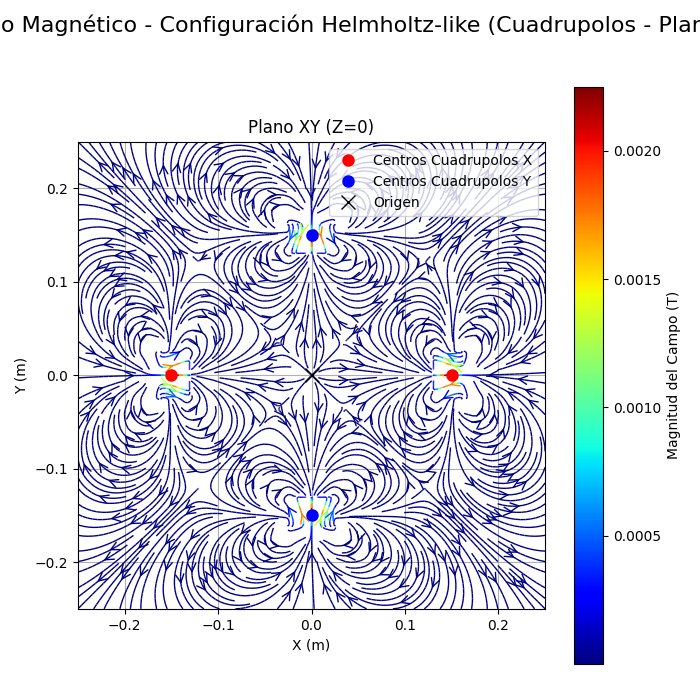
\includegraphics[width=\linewidth, trim={0cm 2cm 0cm 1cm}, clip]{Sections/Figures/helmholtz_quadrupoles_xy_field.png} % Valores de trim/clip de ejemplo
        \caption{Cuadrupolos en Helmholtz.}
        \label{fig:helmholtz_quadrupoles_xy_field}
    \end{minipage}
    \hfill
    \begin{minipage}[b]{0.48\textwidth} % Ancho ajustado
        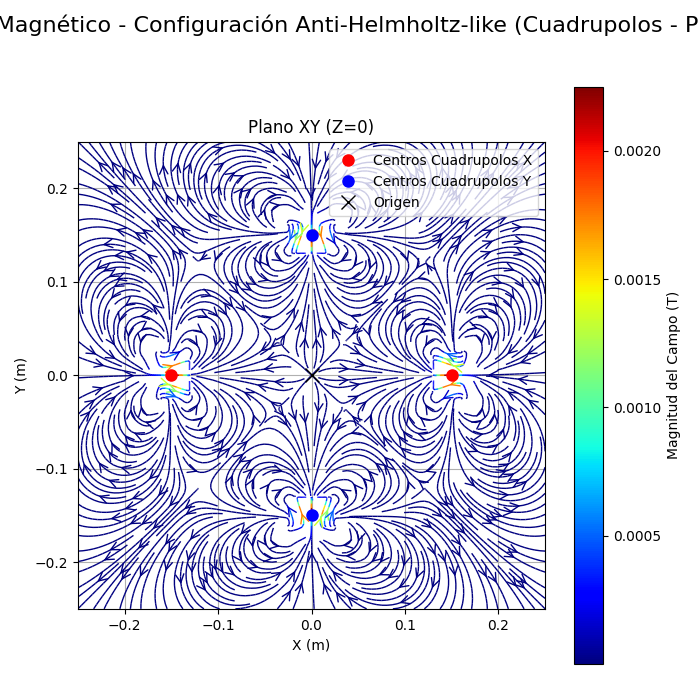
\includegraphics[width=\linewidth, trim={0cm 2cm 0cm 1cm}, clip]{Sections/Figures/antihelmholtz_quadrupoles_xy_field.png} % Valores de trim/clip de ejemplo
        \caption{Cuadrupolos en Anti-Helmholtz.}
        \label{fig:antihelmholtz_quadrupoles_xy_field}
    \end{minipage}
    \caption{Morfología del campo magnético en el plano $x,y$ generado por cuadrupolos en configuraciones Helmholtz y Anti-Helmholtz.}
    \label{fig:campos_cuadrupolos}
\end{figure}

Donde se planeaba fundamentalmente tomar el valor de la \textbf{superposición de estos campos} y multiplicarlo por una expresión periódica que asimilara la variación temporal de las corrientes de las bobinas, de la siguiente forma:

\begin{align*}
\mathbf{B}_{\text{tot}}(\mathbf{r},t) &= \sin(\omega t + \gamma) \, \mathbf{B}_{\text{dipolo}}(\mathbf{r}) \\
\mathbf{B}_{\text{tot}}(\mathbf{r},t) &= \sin(\omega t + \gamma) \, \mathbf{B}_{\text{cuadrupolo}}(\mathbf{r})
\end{align*}

Pero al ver el comportamiento de los campos generados en las imágenes, se llegó a la conclusión de que la mejor forma de simular el sistema era directamente con los \textbf{campos generados por las bobinas}.


\printbibliography

\end{document}
